\chapter{Návrh riešenia}
\section{Meranie hĺbky pamäte samorganizujúcich sa máp}
Ako trénovaciu množinu budem používať sekvenciu písmen abecedy (26 písmen) zostavenú nenáhodným spôsobom (napr. tvoriacu anglické slová z nejakého korpusu).
Vstupmi (trénovacie príklady) pre sieť budú zakódované jednotlivé písmená z trénovacej sekvencie.
Písmená kódujem do 26 prvkového vektora, ktorého prvky budú nuly a jednotka (pre každé písmeno na inej pozícii).
Každý neurón bude mať množinu, v~ktorej si bude pamätať pre aký vstup bol víťazom. Nebude si však ukladať iba konkrétne písmeno zo vstupu, ale $k$ posledných písmen z trénovacej množiny (tzv. sliding window). 
Z toho si viem ďalej vytvoriť hitmapu, ktorá mi bude vizualizovať, na aké vstupy neuróny reagovali.

\begin{figure}[H]
	\centering
	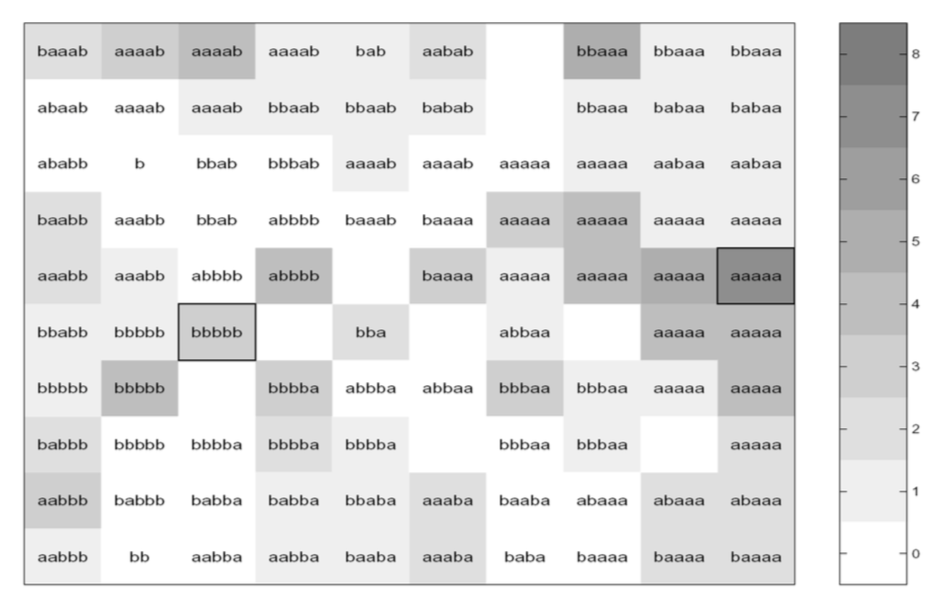
\includegraphics[width=10cm]{assets/receptive_field}
	\caption{Hitmapa}
\end{figure}


Mierou hĺbky pamäte mapy bude potom vážený priemer dĺžky najdlhších spoločných podpostupností písmen v množinách jednotlivých neurónov. Dĺžku najdlhšej podpostupnosti budem určovať od konca sekvencií v množine. Priemer pamäťových hĺbok jednotlivých neurónov musí byť vážený, aby neuróny, %s väčším počtom víťazov mali vyššiu váhu ako neuróny s menším počtom víťazov.
ktoré zvíťazili pre viac vstupov, mali vyššiu váhu ako víťazné neuróny pre menší počet vstupov.
Po každej trénovacej epoche (prechode trénovacou množinou) budem vedieť určiť pamäťovú hĺbku mapy.
Vďaka tomu, že neuróny rekurentných sietí majú okrem normálnych váh aj kontextové váhy, ktoré uchovávajú informáciu z predchádzajúceho kroku,  môže sa stať, že rovnaké písmeno zo vstupu bude mať rôzne víťazné neuróny počas trénovania.


